\chapter{Sprecyzowanie typu generowanych aplikacji} \label{chap:generated_app_type}

Po zebraniu założeń dotyczących rdzenia narzędzia generującego aplikacje, nadszedł czas na wybór typu aplikacji, które będą generowane przez narzędzie.



%=======
\section{Wybór typu aplikacji}
%=======

Narzędzie powinno generować taki typ aplikacji, aby można było w~pełni zbadać jego użyteczność i~ocenić, na ile eliminuje ono duplikację.
Aby było to możliwe, narzędzie powinno generować aplikacje, w~których występuje dużo potencjalnych miejsc występowania duplikacji.

Wymaganie to spełniają aplikacje o~architekturze wielowarstwowej (ang. \emph{multi-tier architecture, n-tier architecture}~\cite{ntier}).


\subsection{Architektura wielowarstwowa}

Architektura wielowarstwowa to taka, w~której ogólne obszary przetwarzania danych w~aplikacji są fizycznie rozdzielone pomiędzy osobne komponenty.
Współpraca pomiędzy tymi komponentami jest zorganizowana w~taki sposób, że komponent $A$ może korzystać z~funkcjonalności komponentu $B$ tylko wtedy, gdy komponent $B$ należy do warstwy logicznie umiejscowionej nie wyżej niż warstwa, do której należy komponent $A$.

Przykładem, a jednocześnie najpopularniejszą realizacją tej architektury jest architektura trójwarstwowa (ang. \emph{three-tier architecture}), która wprowadza podział aplikcji na trzy warstwy:

\begin{enumerate}
 \item Warstwa prezentacji (ang. \emph{Presentation Layer}) - odpowiada za komunikację z~użytkownikiem aplikacji (np. poprzez interfejs graficzny) lub innymi systemami (np. poprzez usługi sieciowe); jest to warstwa logicznie najwyższa;
 \item Warstwa logiki biznesowej (ang. \emph{Business Logic Layer, BLL}) - odpowiada za przetwarzanie danych zgodnie z~wymaganiami funkcjonalnymi aplikacji;
 \item Warstwa dostępu do danych (ang. \emph{Data Access Layer, DAL}) - udostępnia mechanizmy odczytu i~zapisu danych składowanych przez aplikację (np. w~pamięci lub w~bazie danych); jest to warstwa logicznie najniższa.
\end{enumerate}

Współpracę pomiędzy warstwami architektury trójwarstwowej przedstawia diagram zamieszczony na rysunku~\ref{fig:three_tier}.

\begin{figure}[!ht]
 \begin{center}
  \scalebox{0.7}
  {
   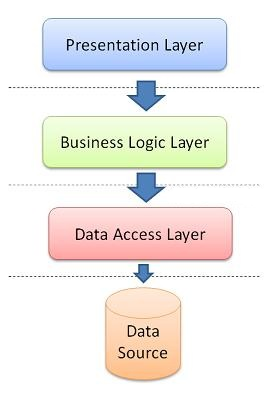
\includegraphics{figures/generated_app_type/three_tier.png}
  }
 \end{center}
 \caption{Współpraca pomiędzy warstwami architektury trójwarstwowej~\cite{three_tier}.}
 \label{fig:three_tier}
\end{figure}


W~takiej architekturze elementy dziedziny aplikacji często mają swoje odwzorowanie w~każdej z~warstw, na przykład:

\begin{itemize}
 \item jako obiekty modelu w~warstwie dostępu do danych;
 \item jako obiekty biznesowe (ang. \emph{business object})~\cite{business_object} w~warstwie logiki biznesowej;
 \item jako modele widoków (ang. \emph{view model})~\cite{view_model} interfejsu użytkownika lub obiekty tranportu danych (ang. \emph{Data Transfer Object, DTO})~\cite{dto} usług sieciowych w~warstwie prezentacji.
\end{itemize}

To sprawia, że aplikacja o~architekturze wielowarstwowej jest narażona na powszechne występowanie duplikacji wiedzy na temat dziedziny aplikacji, a~tym samym dobrze nadaje się jako typ aplikacji generowanych przez narzędzie.



%=======
\section{CQRS}
%=======

Przypadkiem szczególnym architektury wielowarstwowej jest architektura CQRS (\emph{Command Query Responsibility Segregation})~\cite{cqrs_journey}.
Zakłada ona podział wszystkich działań w~aplikacji na dwa rodzaje:

\begin{itemize}
 \item zapytanie (ang. \emph{query}) - działanie polegające na pobraniu danych z~bazy danych (lub innego źródła danych);
 \item komenda (ang. \emph{command}) - działanie polegające na modyfikacji danych w~bazie danych.
\end{itemize}

Działania te w~architekturze CQRS są rozłączne.
Ich wykonywaniem zajmują się dwa osobne modele danych aplikacji:

\begin{itemize}
 \item model zapytań (ang. \emph{Query Model}) - model przeznaczony do odczytu danych;
 \item model komend (ang. \emph{Command Model}) - model przeznaczony do modyfikacji danych.
\end{itemize}

Modele te mogą być całkowicie rozłączne lub częściowo na siebie zachodzić.
Koncepcyjny schemat tej architektury przedstawia rysunek~\ref{fig:cqrs}.

\begin{figure}[!ht]
 \begin{center}
  \scalebox{0.5}
  {
   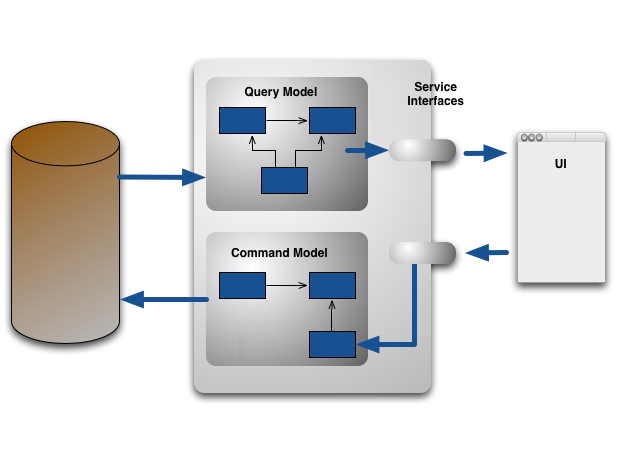
\includegraphics{figures/generated_app_type/cqrs.png}
  }
 \end{center}
 \caption{Schemat architektury CQRS~\cite{cqrs}.}
 \label{fig:cqrs}
\end{figure}


Podział odpowiedzialności pomiędzy komponenty przedstawia się następująco:

\begin{itemize}
 \item model zapytań zajmuje się odczytywaniem danych z~bazy danych;
 \item odpowiedzialnością modelu komend jest realizacja logiki biznesowej aplikacji, w~tym weryfikacja poprawności danych, aktualizacja danych w~bazie danych itd.;
 \item warstwa prezentacji (\emph{UI}):
  \begin{itemize}
   \item wyświetla dane pobrane z~modelu zapytań za pośrednictwem interfejsów (\emph{Service Interfaces}),
   \item przekazuje - w~postaci komend - akcje wykonywane przez użytkownika do modelu komend.
  \end{itemize}
\end{itemize}

Wprowadzenie podziału pomiędzy zapytanie i~komendę niesie ze sobą dwie ważne zalety:

\begin{itemize}
 \item skomplikowana dziedzina aplikacji może być podzielona na dwie prostsze dziedziny, co ułatwia jej zrozumiene i~operowanie na niej;
 \item zapytania i~komendy mogą być wykonywane równolegle, co poprawia wydajność aplikacji;
 \item zapytania są wykonywane na specjalnie przygotowanych dla nich danych (np. zmaterializowanych widokach bazy danych), co ma bardzo pozytywny wpływ na ich wydajność.
\end{itemize}

W~parze z~zaletami idą jednak wady:

\begin{itemize}
 \item synchronizacja obu modeli w~przypadku, gdy korzystają one z~osobnych źródeł danych może być kłopotliwa; problem ten nie występuje na przykład wtedy, gdy model komend operuje na tabelach bazy danych, a~model zapytań - na zmaterializowanych widokach, których źródłem danych są te tabele (synchronizacja modeli odbywa się wtedy automatycznie po stronie bazy danych);
 \item aby każde zapytanie mogło być obsłużone jak najszybciej, model jest w~dużym stopniu zdenormalizowany.
\end{itemize}

Konsekwencją drugiej wady jest to, że w~modelu zapytań masowo występuje duplikacja elementów dziedziny aplikacji.
Jest to dobry powód do tego, aby generator generował aplikacje oparte właśnie o~architekturę CQRS.
Dodatkowo, wybór tej architektury stworzy okazję do przyjrzenia się innym problemom związanym z~zastosowaniem architektury CQRS.
Te problemy to:

\begin{enumerate}
 \item Model komend i model zapytań częściowo na siebie zachodzą lub nawet model zapytań w~całości zawiera model komend - rodzi to dwa pytania:
 \begin{itemize}
  \item jak w~tej sytuacji uniknąć duplikacji wiedzy na temat dziedziny aplikacji?
  \item który model wybrać na “pojedynczą, jednoznaczną i~autorytatywną” (patrz: Zasada ``DRY'' w~rozdziale~\ref{chap:duplication}) reprezentację wiedzy o~dziedzinie aplikacji?
 \end{itemize}
 \item Model komend może nie być nigdzie fizycznie przechowywany - komendy mogą bezpośrednio aktualizować zdenormalizowaną strukturę tabel bazy danych.
 Gdzie w~takim przypadku należy umieścić wiedzę na temat encji należących do dziedziny apliacji?
 Model zapytań nie zawiera przecież encji dziedziny, a~tylko widoki na te encje.
\end{enumerate}

Architektura CQRS często idzie w~parze z~wykorzystaniem wzorca Event Sourcing i~baz danych typu NoSQL.
Zagadnienia te zostaną opisane w~kolejnych sekcjach.



%=======
\section{Event Sourcing}
%=======

Event Sourcing~\cite{eventSourcing_msdn} jest wzorcem architektonicznym, który realizuje przechowywanie stanu aplikacji poprzez przechowywanie wszystkich zdarzeń (ang. \emph{event}), które zaszły w~systemie od początku jego działania aż do stanu obecnego.
Terminem ``zdarzenie'' określa się tutaj dowolną akcję, która ma wpływ na stan systemu.


\subsection{Cechy zdarzenia}

Zdarzenie posiada następujące cechy~\cite{eventSourcing_intro}:

\begin{itemize}
 \item ma ono znaczenie dopiero wtedy, kiedy rzeczywiście wystąpi (np. ``Post został skomentowany'') - zdarzeń przyszłych nie bierze się pod uwagę;
 \item jest ono niezmienne - jako że zdarzenie zaszło w~przeszłości, nie może ono zostać zmienione ani cofnięte; jego skutki mogą jednak zostać zniwelowane przez inne zdarzenie (np. ``Komentarz został usunięty'');
 \item powinno ono mieć znaczenie biznesowe, a~nie implementacyjne - opisanie zajścia zdarzenia słowami: ``Do tabeli Comment dodano nowy rekord'' niesie ze sobą mniejszą wartość biznesową niż: ``Post został skomentowany''.
 \item zazwyczaj zawiera ono informacje na temat kontekstu, w~którym zaszło (np. ``Użytkownik $X$ dodał komentarz $Y$ pod postem $Z$'', ``Moderator $W$ usunął komentarz $Y$'');
 \item informacja o~zajściu zdarzenia jest informacją jednokierunkową od nadawacy (ang. \emph{publisher}) do odbiorcy (ang. \emph{subscriber}) lub wielu odbiorców; reakcja odbiorcy na zdarzenie nie jest bezpośrednio znana nadawcy.\\
\end{itemize}

Rejestrowanie zdarzeń odbywa się poprzez stworzenie obiektu opisującego daną akcję i~zapisanie go w~systemie.
Zdarzenia rejestrowane są w~dzienniku zdarzeń (ang. \emph{event log} lub \emph{event storage}).
Za reagowanie na zdarzenia, a~w~efekcie faktyczną zmianę stanu systemu odpowiadają wyznaczone do tego obiekty implementujące odpowiednie procedury obsługi (ang. \emph{event handlers}).
Obiekty te pobierają nieprzetworzone zdarzenia z~dziennika zdarzeń i~wykonują procedury.
Pojedyczne zdarzenie może zostać przetworzone przez wiele takich obiektów, wykonujących wiele osobnych modyfikacji stanu systemu.


\subsection{Zalety i~wady wzorca}

Wzorzec Event Sourcing wprowadza nastepujące zalety:

\begin{itemize}
 \item dziennik zdarzeń dostarcza informacji o~historii działań użytkoniwków systemu - informacje te mogą być przydatne podczas szukania przyczyn występienia błędów;
 \item aplikację można łatwo usunąć i~przywrócić do poprzedniego stanu poprzez zarejestrowanie wszystkich zdarzeń od nowa (np. podczas przenoszenia jej na inną maszynę);
 \item stan aplikacji można łatwo cofnąć do dowolnego punktu w~czasie - wystarczy wyczyścić stan aplikacji i~zarejestrować od nowa wszystkie zdarzenia, ktore zaszły przed wybranym punktem w~czasie (może to ułatwić szukanie przyczyn wystąpienia błędów);
 \item w~razie wykrycia zdarzenia będącego przyczyną wystąpienia błędu, można usunąć to zdarzenie z~dziennika i~zarejestrować od nowa wszystkie zdarzenia, które nastąpiły po nim; na podobnej zasadzie można skorygować kolejność zdarzeń zarejestowanych w~złej kolejności (z~tej zalety powinno się korzystać jedynie w~sytuacjach awaryjnych, ponieważ narusza ona cechę zdarzeń mówiącą o~ich niezmieności).
\end{itemize}

Wady:

\begin{itemize}
 \item implementacja dziennika zdarzeń nie jest łatwa - powinna ona gwarantować, że zdarzenia zostaną wpisane do dziennika w~kolejności ich zgłaszania (co nie jest oczywiste w~aplikacjach wielowątkowych);
 \item z~reguły reakcja na zdarzenie odbywa się asynchronicznie względem procesu zgłaszającego jego zajście - zmiany stanu systemu nie są więc widoczne natychmiast po zajściu zdarzenia; zjawisko to jest widoczne na przykład w~serwisie YouTube~\cite{youtube} - zdarzenie ``Obejrzano film'' jest przetwarzane znacznie wolniej niż zdarzenie ``Dodano komentarz'' (wyświetlenia filmu sprawdzane są pod kątem fałszywych wyświetleń mających na celu sztuczne zwiększenie popularności filmu~\cite{youtube:301}), co skutkuje wyświetleniem większej liczby komentarzy niż liczby wyświetleń pod danym filmem (jeśli komentarzy i~wyświetleń jest odpowiednio dużo);
 \item odtwarzanie stanu systemu, w~którym zarejestrowano tysiące zdarzeń może trwać bardzo długo (rozwiązaniem tego problemu jest tworzenie migawek (ang. \emph{snapshot}) systemu przechowujacych stan systemu co ileś zdarzeń);
 \item zmiany w~kodzie źródłowym systemu moga powodować, że dawno zarejestrowane zdarzenia przestaną być niekompatybilne z~nową wersją systemu.
\end{itemize}


\subsection{Przykłady aplikacji wykorzystujących Event Sourcing}

Aby łatwiej zrozumieć działanie wzorca, garść przykładów aplikacji używanych na co dzień, które są oparte o~Event Sorcing lub częściowo go wykorzystują:

\begin{itemize}
 \item systemy kontroli wersji - dziennik zdarzeń przechowuje zmiany dokonywane na plikach znajdujących się w~wersjonowanym katalogu;
 \item edytory tekstu i~edytory graficzne - dziennik zdarzeń przechowuje zmiany dokonywane na edytowanym pliku.
\end{itemize}

Wzorzec ten ma jednak zastosowanie nie tylko w~aplikacjach użytkowych.
W~połączeniu z~wzorcem CQRS, sprawdza się także w~aplikacjach klasy enterprise.


\subsection{Współpraca z~CQRS}

Zasady działania wzorca Event Sorcing w~systemie opartym o~architekturę CQRS są następujące~\cite{cqrs_es}:

\begin{itemize}
 \item rolę modelu komend pełni dziennik zdarzeń - jedynym zadaniem komend jest zarejestrowanie zdarzenia w~dzienniku;
 \item stan systemu jest przechowywany w~modelu zapytań;
 \item za synchronizację modelu zapytań z~modelem komend odpowiadają procedury obsługi zdarzeń (\emph{event handlers}) - synchronizacja ta odbywa się asynchronicznie;
 \item wzorzec Event Sourcing nie ma wpływu na warstwę prezentacji systemu.
\end{itemize}


Współpraca ta została schematycznie przedstawiona na rysunku~\ref{fig:cqrs_es}.

\begin{figure}[!ht]
 \begin{center}
  \scalebox{0.6}
  {
   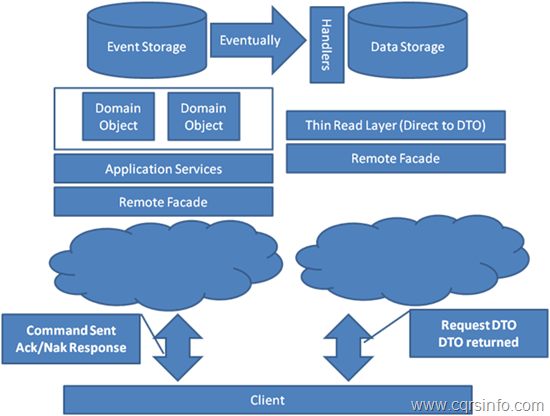
\includegraphics{figures/generated_app_type/cqrs_es.png}
  }
 \end{center}
 \caption{Współpraca wzorca Event Sourcing z~architekturą CQRS~\cite{cqrs_info}.}
 \label{fig:cqrs_es}
\end{figure}




%=======
\section{NoSQL}
%=======

Bazy danych typu NoSQL (ang. \emph{Not Only SQL}) odrzucają praktykę składowania danych w~tabelarycznej, opartej na relacjach, ustrukturyzywanej formie będącej podstawą relacyjnych baz danych.
Zamiast tego składują dane w~innych, bardziej elastycznych postaciach, na przykład grafu lub zbioru par klucz-wartość.
Pozwala to na wykonywanie niektórych operacji szybciej, niż są one wykonywane przez relacyjne bazy danych.
Nie jest to jednak rozwiązanie bezwględnie lepsze od relacyjnych baz danych - niektóre operacje są wykonywane wolniej w~bazach typu NoSQL, niż w~bazach relacyjnych.

Bazy danych typu NoSQL są nastawione na przechowywanie bardzo dużych ilości danych.
Tym, co odróżnia je od baz relacyjnych jest fakt, że zazwyczaj domyślnie wspierają one rozproszenie danych pomiędzy wiele maszyn.
Zapewnia to łatwą poziomą skalowalność systemów z~nich korzystających.


\subsection{Dostępne bazy NoSQL}

Bazy danych typu NoSQL są tworzone pod kątem konkretnych problemów, jakie mają rozwiązywać.
Dlatego istnieje wiele takich baz, które różnią się wydajnością bądź oferowanymi funkcjonalnościami.
Można je podzielić ze względu na model przechowywania danych.
Najczęściej stosowane modele to:

\subsubsection{Rodzina kolum}

Rodzina kolumn (ang. \emph{column family}, \emph{wide column}) jest modelem najbardziej przypominającym tabele w~relacyjnej bazie danych.
Dane przechowywane są w~wierszach, które składają się z~kolumn wraz z~przypisanymi im wartościami.
Pojedyczny wiersz może składać się z~bardzo dużej liczby kolumn.
W~odróżnieniu od relacyjnych baz danych, wiersz nie musi posiadać wszystkich kolumn wchodzących w~skład rodziny i~może posiadać kolumny nienalażące do rodziny.
Każda wartość przypisana do dajen kolumny wchodzącej w~skład rodziny musi jednak być określonego dla tej kolumny typu.

W~odróżnieniu od baz relacyjnych bazy oparte o~rodziny kolumn nie~wspierają relacji pomiędzy tabelami (rodzinami kolumn).
Aby osiągnąć satyfakcjonującą wydajność przeszukiwania, przechowuje się w~nich dane o~wysokim stopniu denormalizacji.
Przykłady baz danych przechowujących rodziny kolumn:

\begin{itemize}
 \item Hadoop~\cite{hadoop} - platforma stworzona w~technologii Java, wykonująca obliczenia na dużych ilościach danych realizowane przez wiele rozproszonych aplikacji, służy przede wszstkim do przetwarzania danych, a~nie do ich składowania;
 \item Cassandra~\cite{cassandra} - stworzona w~technologii Java baza danych, której główne cele to skalowalność, wysoka wydajność i~brak pojedynczego punktu awarii (ang. \emph{Single Point of Failure}, \emph{SPOF});
 \item Amazon SimpleDB~\cite{simple_db} - komercyjna baza danych nastawiona na prostotę użytkowania i~zarządzania.
\end{itemize}

\subsubsection{Zbiór par klucz-wartość}

Para klucz-wartość (ang. \emph{key-value pair}) jest zdecydowanie najprostszą strukturą danych używaną w~bazach danych typu NoSQL.
Przechowywane w~postaci zbiorów takich par dane nie są w~żaden sposób ustrukturyzywane.
Pary klucz-wartość są podstawą dla innych modeli danych, na przykład rodzin kolumn, gdzie wiersze składają się z~par kolumna-wartość.
Są więc najbardziej elastycznym modelem, ale zazwyczaj oferującym ubogi zestaw funkcjonalności.

Przykłady baz przechowujących pary klucz-wartość to:

\begin{itemize}
 \item DynamoDB~\cite{dynamo_db} - baza danych będąca w~stanie wydajnie działać pod bardzo dużym obciążeniem, jej kluczowymi celami są wydajność i~skalowalność; stworzona w~technologii Java;
 \item Azure Table Storage~\cite{azure_table_storage} - baza danych wspierająca przchowywanie danych w~tabelarycznej, ustrukturyzywanej formie; stworzona na platformie .Net;
 \item Redis~\cite{redis} - napisana w~języku C wydajna baza danych wspierająca przechowywanie złożonych struktur takich jak listy, kolejki czy posortowane zbiory.
\end{itemize}

\subsubsection{Graf}

Niektóre bazy danych typu NoSQL za model danych obierają graf.
Takie bazy nazywamy grafowymi bazami danych (ang. \emph{graph databases}).

Węzłem grafu może być dowolny obiekt (np. zbiór par klucz-wartość), a~krawędź może łączyć dwa dowolne węzły.
Pojedyncza krawędź reprezentuje dowolną relację pomiędzy węzłami.
Model ten jest więc bardzo elastyczny.

Zaletą grafu jest to, że, podobnie jak relacja, jest on strukturą danych o~silnym podłożu matematycznym.
Istnieje więc wiele wydajnych algorytmów operujących na tej strukturze (np. algorytmy wyszukiwania ścieżek), co sprawia, że struktura ta bardzo dobrze nadaje się do modelowania wszelkiego rodzaju danych przestrzennych (np. map) lub innych sieci (np. zbiorów użytkowników portali społecznościowych, gdzie wierzchołek reprezentuje osobę, a~krawędź - relację ``zna'').

Do grafowych baz danych należą:

\begin{itemize}
 \item Neo4J~\cite{neo4j} - najpopularniejsza grafowa baza danych, cechuje się wysoką wydajnością i~skalowalnością; wspiera mechanizm transakcji; stworzona w~technologii Java;
 \item TITAN~\cite{titan} - baza danych wykorzystująca inne rozwiązania, takie jak Cassandra, korzytając z~wymiennych mechanizmów; stworzona w~technologii Java;
 \item Trinity~\cite{trinity} - stworzona na platformie .Net baza danych wspierająca wygodne, deklaratywne modelowanie i~przeszukiwanie danych.
\end{itemize}

\subsubsection{Dokument}

Dokument (ang. \emph{document}) jest typem danych, który z~założenia reprezentuje duże porcje danych, z~których tylko fragmenty są udostępniane na potrzeby pojedynczych zapytań.
Dokumenty mogą posiadać dowolną strukturę, na co pozwala format, w~jakim są przechowywane (np. XML lub JSON).

Bazy danych przechowujace dokumenty (ang. \emph{document-oriented databases}) są więc przystosowane do przechowywania i~przeszukiwania dużych jednostek danych.
Do baz tego rodzaju należą:

\begin{itemize}
 \item MongoDB~\cite{mongo_db} - umożliwia wygodne przeszukiwanie danych i~tworzenie indeksów na dowolnych ich atrybutach, wspiera automatyczne dzielenie danych pomiędzy wiele maszyn (ang. \emph{sharding}); stworzona w~języku C++;
 \item CouchDB~\cite{couch_db} - stworzona w~języku Erlang baza danych udostępniająca przechowywane dane poprzez protokół HTTP; nastawiona na wykorzystanie w~aplikacjach webowych i~mobilnych;
 \item RavenDB~\cite{raven_db} - baza danych umożliwiająca wykonywanie dowolnych operacji (np. przebudowy struktury) bez potrzeby zatrzymywania korzystających z~niej aplikacji i~udostępniająca wygodny sposób przeszukiwania danych; oparta na platformie .Net.
\end{itemize}


\subsection{Dlaczego Cassandra}

Spośród dostępnych rodzajów baz danych typu NoSQL należy wybrać jeden, który będzie używany przez aplikacje generowane przez narzędzie.


Że rodziny kolumn.
Bo najbardziej zblizone do rdbms, więc najwygodniej w nich modelować dziedzinę dowolnej apliakacji.
(mogłyby też być document-oriented, ale typowo przechowywane obiekty nie będą aż tak duże)

Jak to będzie współgrać z CQRS + ES (zdarzenia (model komend) przechowywane gdziekolwiek (rdbms lub nosql), ale skupimy się na modelu zapytań) - który będzie ostro zdenormalizowany, więc dobrze nadaje się pod rodziny kolumn

wybrać bazę NoSQL i dlaczego Cassandra (bo najpopularniejsza, najbardziej wydajna)



%=======
\section{Cassandra}
%=======

opisać Cassandrę
